\subsection{Hello Triangle}

In OpenGL everything is in 3D space, but the screen or window is a 2D array of pixels so a large part of OpenGL's work is about transforming all 3D coordinates to 2D pixels that fit on your screen. The process of transforming 3D coordinates to 2D pixels is managed by the \textbf{graphics pipeline} of OpenGL. The graphics pipeline can be divided into two large parts: the first transforms your 3D coordinates into 2D coordinates and the second part transforms the 2D coordinates into actual colored pixels. In this chapter we'll briefly discuss the graphics pipeline and how we can use it to our advantage to create fancy pixels.

The graphics pipeline takes as input a set of 3D coordinates and transforms these to colored 2D pixels on your screen. The graphics pipeline can be divided into several steps where each step requires the output of the previous step as its input. All of these steps are highly specialized (they have one specific function) and can easily be executed in parallel. Because of their parallel nature, graphics cards of today have thousands of small processing cores to quickly process your data within the graphics pipeline. The processing cores run small programs on the GPU for each step of the pipeline. These small programs are called shaders.

Some of these shaders are configurable by the developer which allows us to write our own shaders to replace the existing default shaders. This gives us much more fine-grained control over specific parts of the pipeline and because they run on the GPU, they can also save us valuable CPU time. Shaders are written in the \textbf{OpenGL Shading Language (GLSL)} and we'll delve more into that in the next chapter.

Below you'll find an abstract representation of all the stages of the graphics pipeline. Note that the blue sections represent sections where we can inject our own shaders.

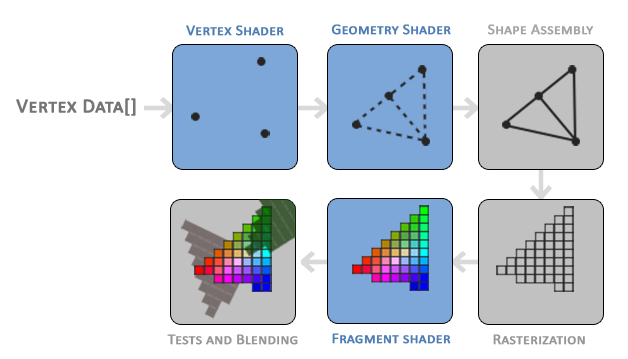
\includegraphics[scale = 2.5]{pics/pipeline.png}

As you can see, the graphics pipeline contains a large number of sections that each handle one specific part of converting your vertex data to a fully rendered pixel. We will briefly explain each part of the pipeline in a simplified way to give you a good overview of how the pipeline operates.

As input to the graphics pipeline we pass in a list of three 3D coordinates that should form a triangle in an array here called \verb|Vertex Data|; this vertex data is a collection of vertices. A vertex is a collection of data per 3D coordinate. This vertex's data is represented using vertex attributes that can contain any data we'd like, but for simplicity's sake let's assume that each vertex consists of just a 3D position and some color value.

\begin{note}
    In order for OpenGL to know what to make of your collection of coordinates and color values OpenGL requires you to hint what kind of render types you want to form with the data. Do we want the data rendered as a collection of points, a collection of triangles or perhaps just one long line? Those hints are called primitives and are given to OpenGL while calling any of the drawing commands. Some of these hints are \verb|GL_POINTS|, \verb|GL_TRIANGLES| and \verb|GL_LINE_STRIP|.
\end{note}

\begin{center}
    \textbf{Vertex Shader}\\
    The first part of the pipeline is the vertex shader that takes as input a single vertex. The main purpose of the vertex shader is to transform 3D coordinates into different 3D coordinates (more on that later) and the vertex shader allows us to do some basic processing on the vertex attributes.
\end{center}

\begin{center}
    \textbf{Geometry Shader}\\
    The output of the vertex shader stage is optionally passed to the geometry shader. The geometry shader takes as input a collection of vertices that form a primitive and has the ability to generate other shapes by emitting new vertices to form new (or other) primitive(s). In this example case, it generates a second triangle out of the given shape.
\end{center}

\newpage

\begin{center}
    \textbf{Primitive Assembly}\\
    The primitive assembly stage takes as input all the vertices (or vertex if \verb|GL_POINTS| is chosen) from the vertex (or geometry) shader that form one or more primitives and assembles all the point(s) in the primitive shape given; in this case two triangles.
\end{center}

\begin{center}
    \textbf{Rasterization Stage}\\
    The output of the primitive assembly stage is then passed on to the rasterization stage where it maps the resulting primitive(s) to the corresponding pixels on the final screen, resulting in fragments for the fragment shader to use. Before the fragment shaders run, clipping is performed. \textbf{Clipping} discards all fragments that are outside your view, increasing performance.
\end{center}

\begin{center}
    \textbf{Fragment Shader}\\
    The main purpose of the fragment shader is to calculate the final color of a pixel and this is usually the stage where all the advanced OpenGL effects occur. Usually the fragment shader contains data about the 3D scene that it can use to calculate the final pixel color (like lights, shadows, color of the light and so on).
\end{center}

\begin{center}
    \textbf{Alpha Tests and Blending Stage}\\
    After all the corresponding color values have been determined, the final object will then pass through one more stage that we call the \textbf{alpha test} and \textbf{blending} stage. This stage checks the corresponding depth (and stencil) value (we'll get to those later) of the fragment and uses those to check if the resulting fragment is in front or behind other objects and should be discarded accordingly. The stage also checks for alpha values (alpha values define the opacity of an object) and blends the objects accordingly. So even if a pixel output color is calculated in the fragment shader, the final pixel color could still be something entirely different when rendering multiple triangles.
\end{center}

As you can see, the graphics pipeline is quite a complex whole and contains many configurable parts. However, for almost all the cases we only have to work with the \textbf{vertex} and \textbf{fragment} shader. The geometry shader is optional and usually left to its default shader.

In modern OpenGL we are \textbf{required} to define at least a vertex and fragment shader of our own (there are no default vertex/fragment shaders on the GPU). For this reason it is often quite difficult to start learning modern OpenGL since a great deal of knowledge is required before being able to render your first triangle. Once you do get to finally render your triangle at the end of this chapter you will end up knowing a lot more about graphics programming.

To start drawing something we have to first give OpenGL some input vertex data. OpenGL is a 3D graphics library so all coordinates that we specify in OpenGL are in 3D ($x$, $y$ and $z$ coordinate). OpenGL doesn't simply transform all your 3D coordinates to 2D pixels on your screen; OpenGL only processes 3D coordinates when they're in a specific range between -1.0 and 1.0 on all 3 axes ($x$, $y$ and $z$). All coordinates within this so called \textbf{normalized device coordinates} range will end up visible on your screen (and all coordinates outside this region won't).

Because we want to render a single triangle we want to specify a total of three vertices with each vertex having a 3D position. We define them in normalized device coordinates (the visible region of OpenGL) in a float array:

\newpage

\begin{lstlisting}[language=C++]
    float vertices[] = {
        -0.5f, -0.5f, 0.0f,
        0.5f, -0.5f, 0.0f,
        0.0f,  0.5f, 0.0f
    };  
\end{lstlisting}

Because OpenGL works in 3D space we render a 2D triangle with each vertex having a $z$ coordinate of 0.0. This way the depth of the triangle remains the same making it look like it's 2D.

\begin{note}
    \begin{center}
        \textbf{Normalized Device Coordinates (NDC)}
    \end{center}
    Once your vertex coordinates have been processed in the vertex shader, they should be in normalized device coordinates which is a small space where the $x$, $y$ and $z$ values vary from -1.0 to 1.0. Any coordinates that fall outside this range will be discarded/clipped and won't be visible on your screen. Below you can see the triangle we specified within normalized device coordinates (ignoring the $z$ axis):

    \begin{center}
        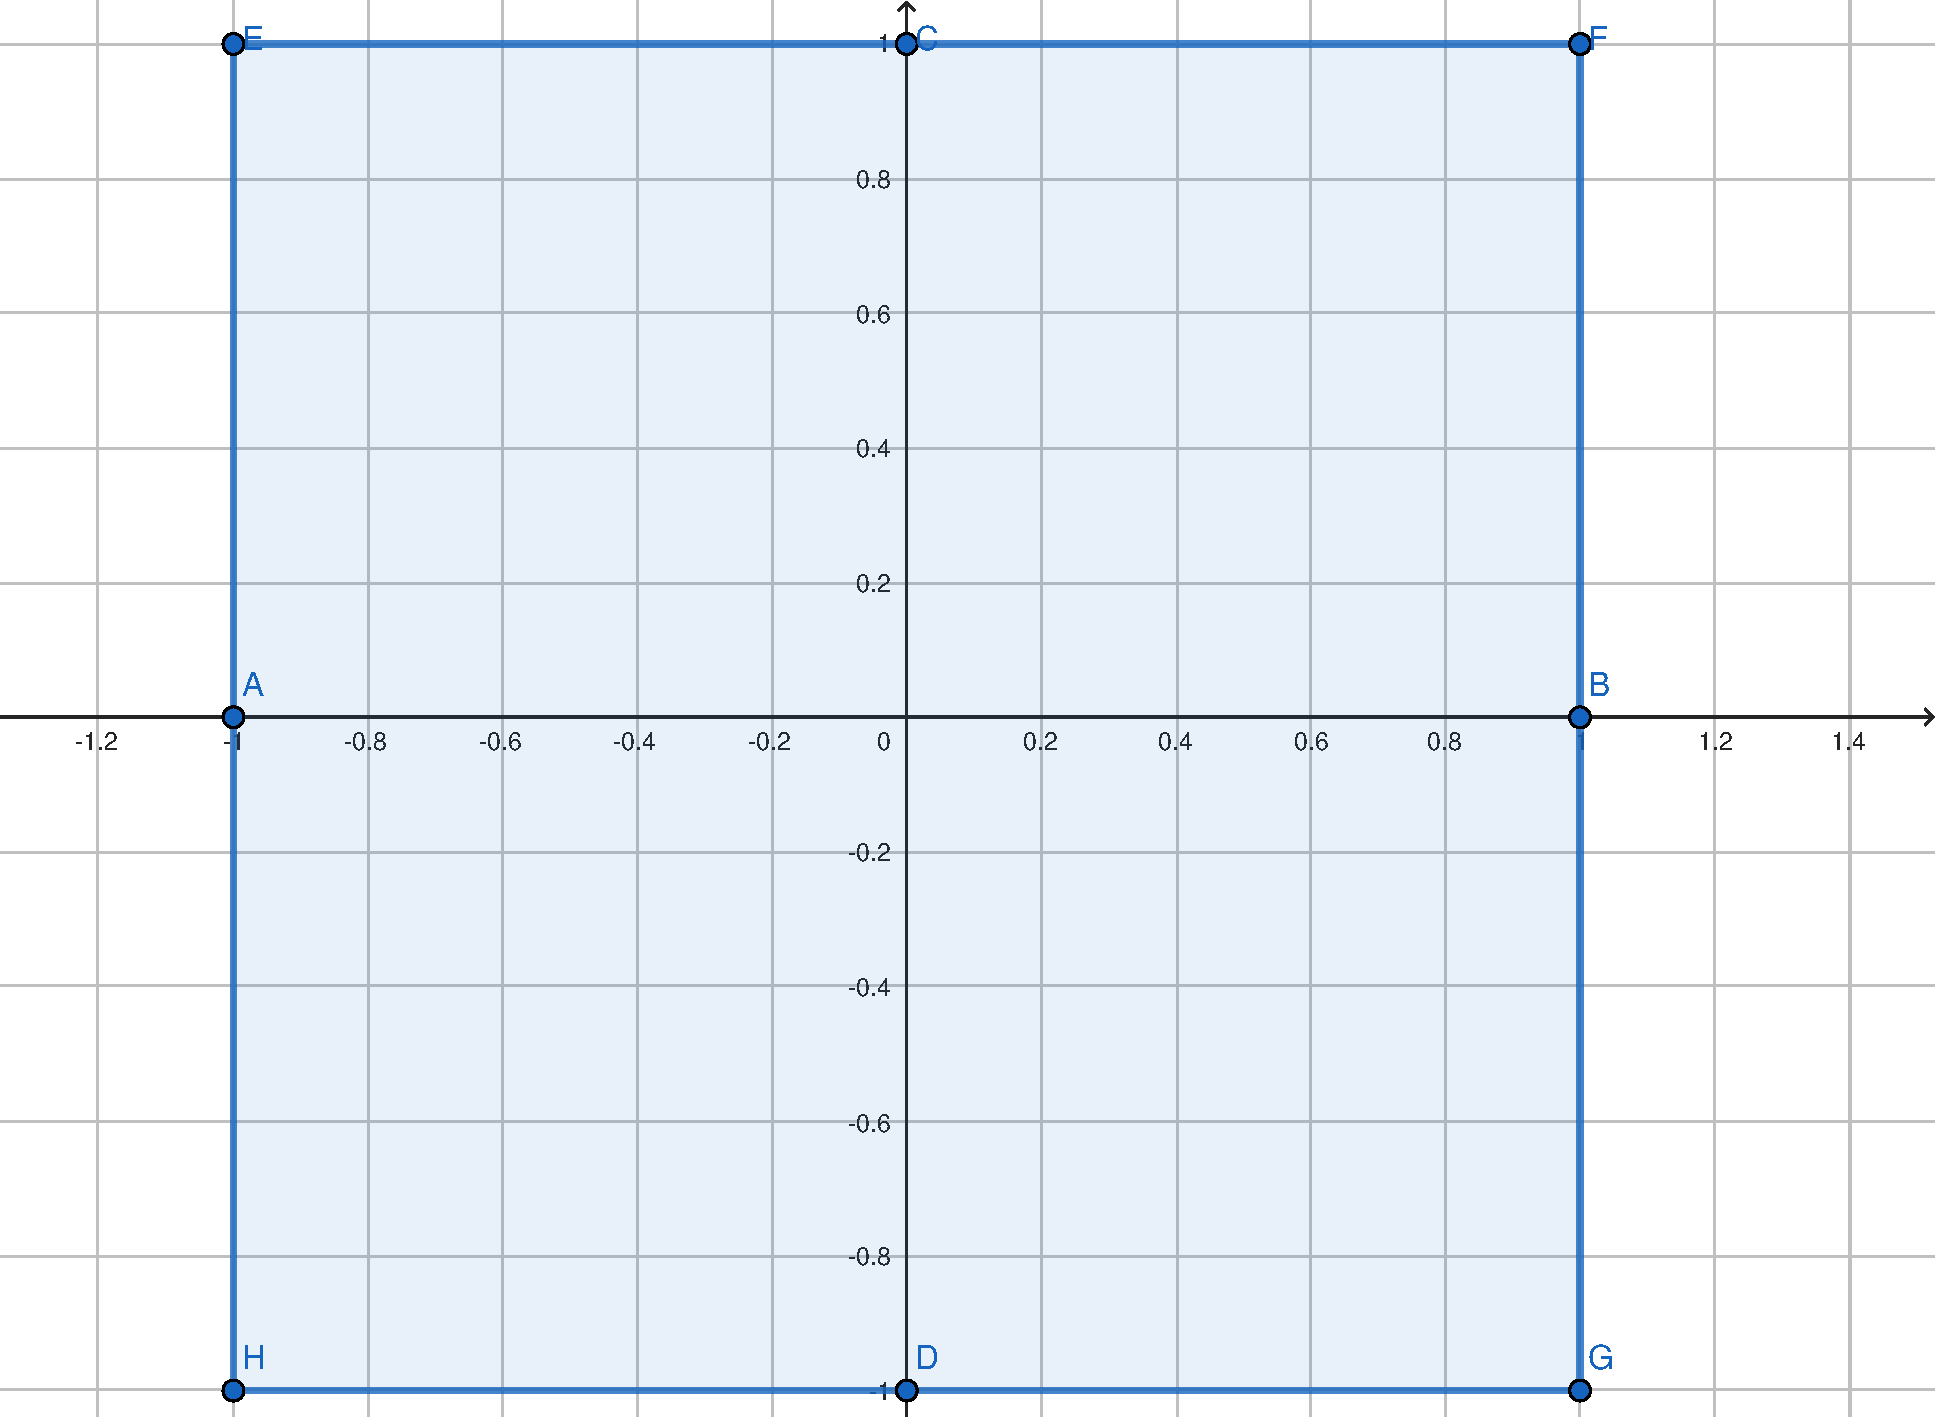
\includegraphics[scale=0.4]{pics/bounds.pdf}
    \end{center}

    \begin{center}
        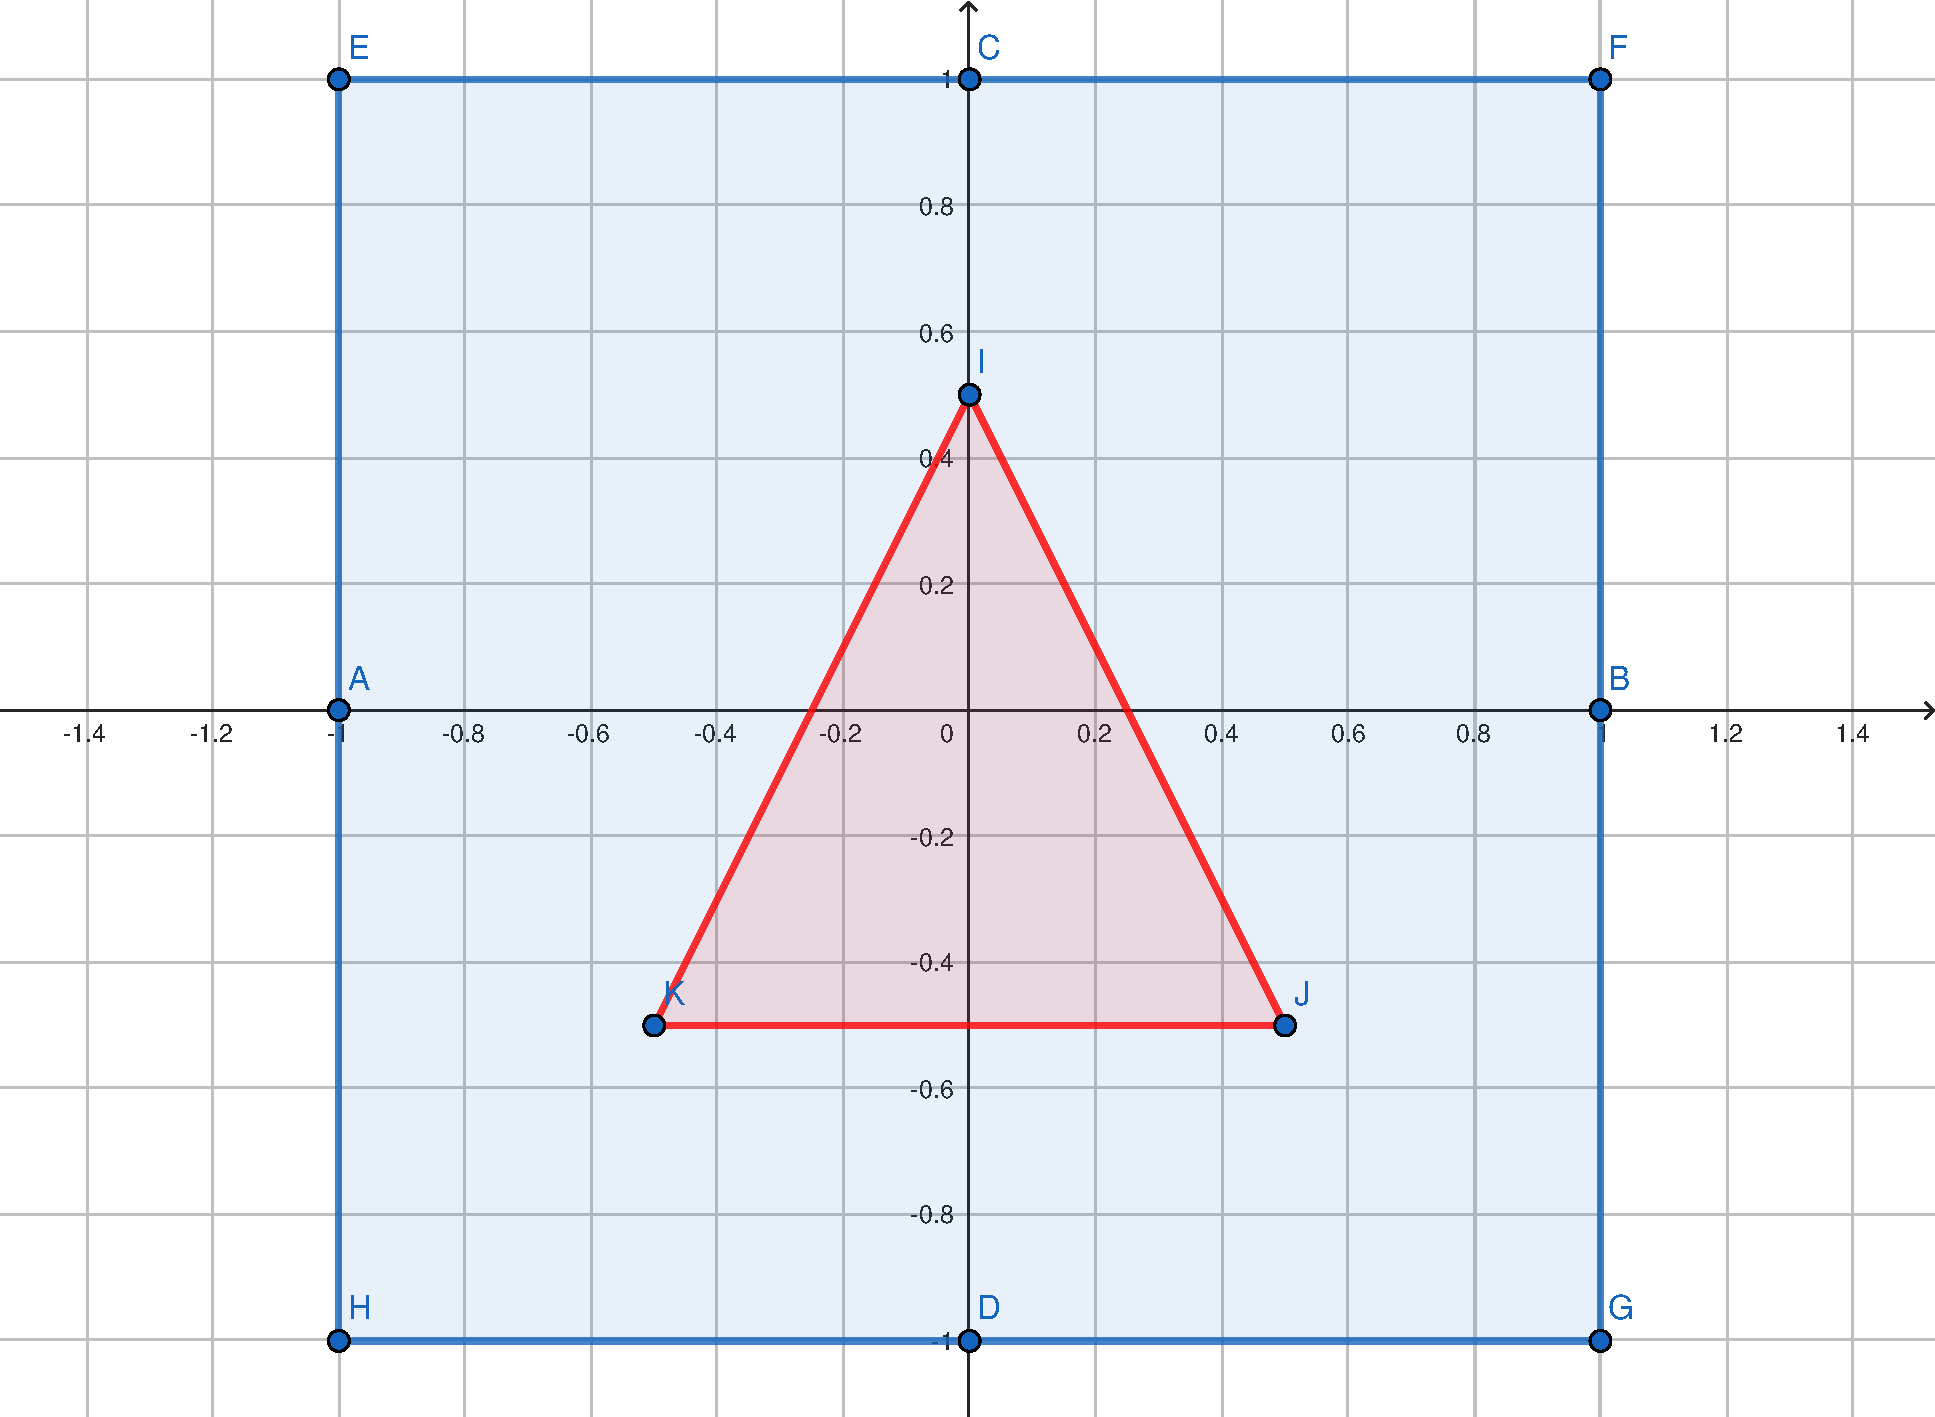
\includegraphics[scale=0.4]{pics/triangle_ndc.pdf}
    \end{center}

    Unlike usual screen coordinates the positive $y$-axis points in the up-direction and the (0,0) coordinates are at the center of the graph, instead of top-left. Eventually you want all the (transformed) coordinates to end up in this coordinate space, otherwise they won't be visible.

    Your NDC coordinates will then be transformed to screen-space coordinates via the viewport transform using the data you provided with \verb|glViewport|. The resulting screen-space coordinates are then transformed to fragments as inputs to your fragment shader.
\end{note}

With the vertex data defined we'd like to send it as input to the first process of the graphics pipeline: the vertex shader. This is done by creating memory on the GPU where we store the vertex data, configure how OpenGL should interpret the memory and specify how to send the data to the graphics card. The vertex shader then processes as much vertices as we tell it to from its memory.

We manage this memory via so called \textbf{vertex buffer objects (VBO)} that can store a large number of vertices in the GPU's memory. The advantage of using those buffer objects is that we can send large batches of data all at once to the graphics card, and keep it there if there's enough memory left, without having to send data one vertex at a time. Sending data to the graphics card from the CPU is relatively slow, so wherever we can we try to send as much data as possible at once. Once the data is in the graphics card's memory the vertex shader has almost instant access to the vertices making it extremely fast.

Just like any object in OpenGL, this buffer has a unique ID corresponding to that buffer, so we can generate one with a buffer ID using the \verb|glGenBuffers| function:

\newpage

\begin{lstlisting}[language=C++]
    unsigned int VBO;
    glGenBuffers(1, &VBO);
\end{lstlisting}

OpenGL has many types of buffer objects and the buffer type of a vertex buffer object is \verb|GL_ARRAY_BUFFER|. OpenGL allows us to bind to several buffers at once as long as they have a different buffer type. We can bind the newly created buffer to the \verb|GL_ARRAY_BUFFER| target with the \verb|glBindBuffer| function:

\begin{lstlisting}[language=C++]
    glBindBuffer(GL_ARRAY_BUFFER, VBO);
\end{lstlisting}

From that point on any buffer calls we make (on the \verb|GL_ARRAY_BUFFER| target) will be used to configure the currently bound buffer, which is VBO. Then we can make a call to the \verb|glBufferData| function that copies the previously defined vertex data into the buffer's memory:

\begin{lstlisting}[language=C++]
    glBufferData(GL_ARRAY_BUFFER, sizeof(vertices), vertices, GL_STATIC_DRAW);
\end{lstlisting}

\verb|glBufferData| is a function specifically targeted to copy user-defined data into the currently bound buffer. Its first argument is the type of the buffer we want to copy data into: the vertex buffer object currently bound to the \verb|GL_ARRAY_BUFFER| target. The second argument specifies the size of the data (in bytes) we want to pass to the buffer; a simple \verb|sizeof| of the vertex data suffices. The third parameter is the actual data we want to send.
The fourth parameter specifies \textbf{how we want the graphics card to manage the given data}. This can take 3 forms:

\begin{itemize}
    \item \verb|GL_STREAM_DRAW|: the data is set only once and used by the GPU at most a few times.
    \item \verb|GL_STATIC_DRAW|: the data is set only once and used many times.
    \item \verb|GL_DYNAMIC_DRAW|: the data is changed a lot and used many times.
\end{itemize}

The position data of the triangle does not change, is used a lot, and stays the same for every render call so its usage type should best be \verb|GL_STATIC_DRAW|. If, for instance, one would have a buffer with data that is likely to change frequently, a usage type of \verb|GL_DYNAMIC_DRAW| ensures the graphics card will place the data in memory that allows for faster writes.

As of now we stored the vertex data within memory on the graphics card as managed by a vertex buffer object named VBO. Next we want to create a vertex and fragment shader that actually processes this data, so let's start building those.

The first thing we need to do is write the vertex shader in the shader language GLSL (OpenGL Shading Language) and then compile this shader so we can use it in our application. Below you'll find the source code of a very basic vertex shader in GLSL:

\begin{lstlisting}[language=C++]
    #version 330 core
    layout (location = 0) in vec3 aPos;

    void main()
    {
        gl_Position = vec4(aPos.x, aPos.y, aPos.z, 1.0);
    }
\end{lstlisting}